\section{Basic assumptions}
The whole project is designed based on two basic assumptions: (1) social media data can be used to predict the outbreak of diseases; (2) available data contain sufficient information to show the relationship between input and output.

\section{Overall design}
\label{sec:Overall design}
Generally, our system can be divided into two components: (1) signal extracting: extract healthcare-related topics from social media; (2) modeling: build a predictive model based on extracted signals. Treat our system as a Blackbox, the input is the metadata extracted from social media platforms while the output is the prediction of diseases (Figure \ref{fig:sys1}). 
\begin{figure}[!htp]
    \center
    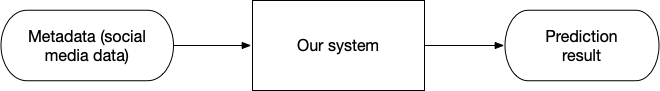
\includegraphics[width=5in]{images/system1.png}
    \caption{Blackbox}
    \label{fig:sys1}
\end{figure}
\\The aims of overall design involve building a complete process where the performance is reproducible, the subprocesses can be adjusted and the outcome can be easily understood and visualized. Based on it, we separate the Blackbox into 6 independent components: Data Collector, Preprocessor, Classification Model, Clustering Model, Evaluation layer, visualization. The overall structure can be seen in Figure \ref{fig:sys2}, the square represents component while ellipse represents data.
\begin{figure}[!htp]
    \center
    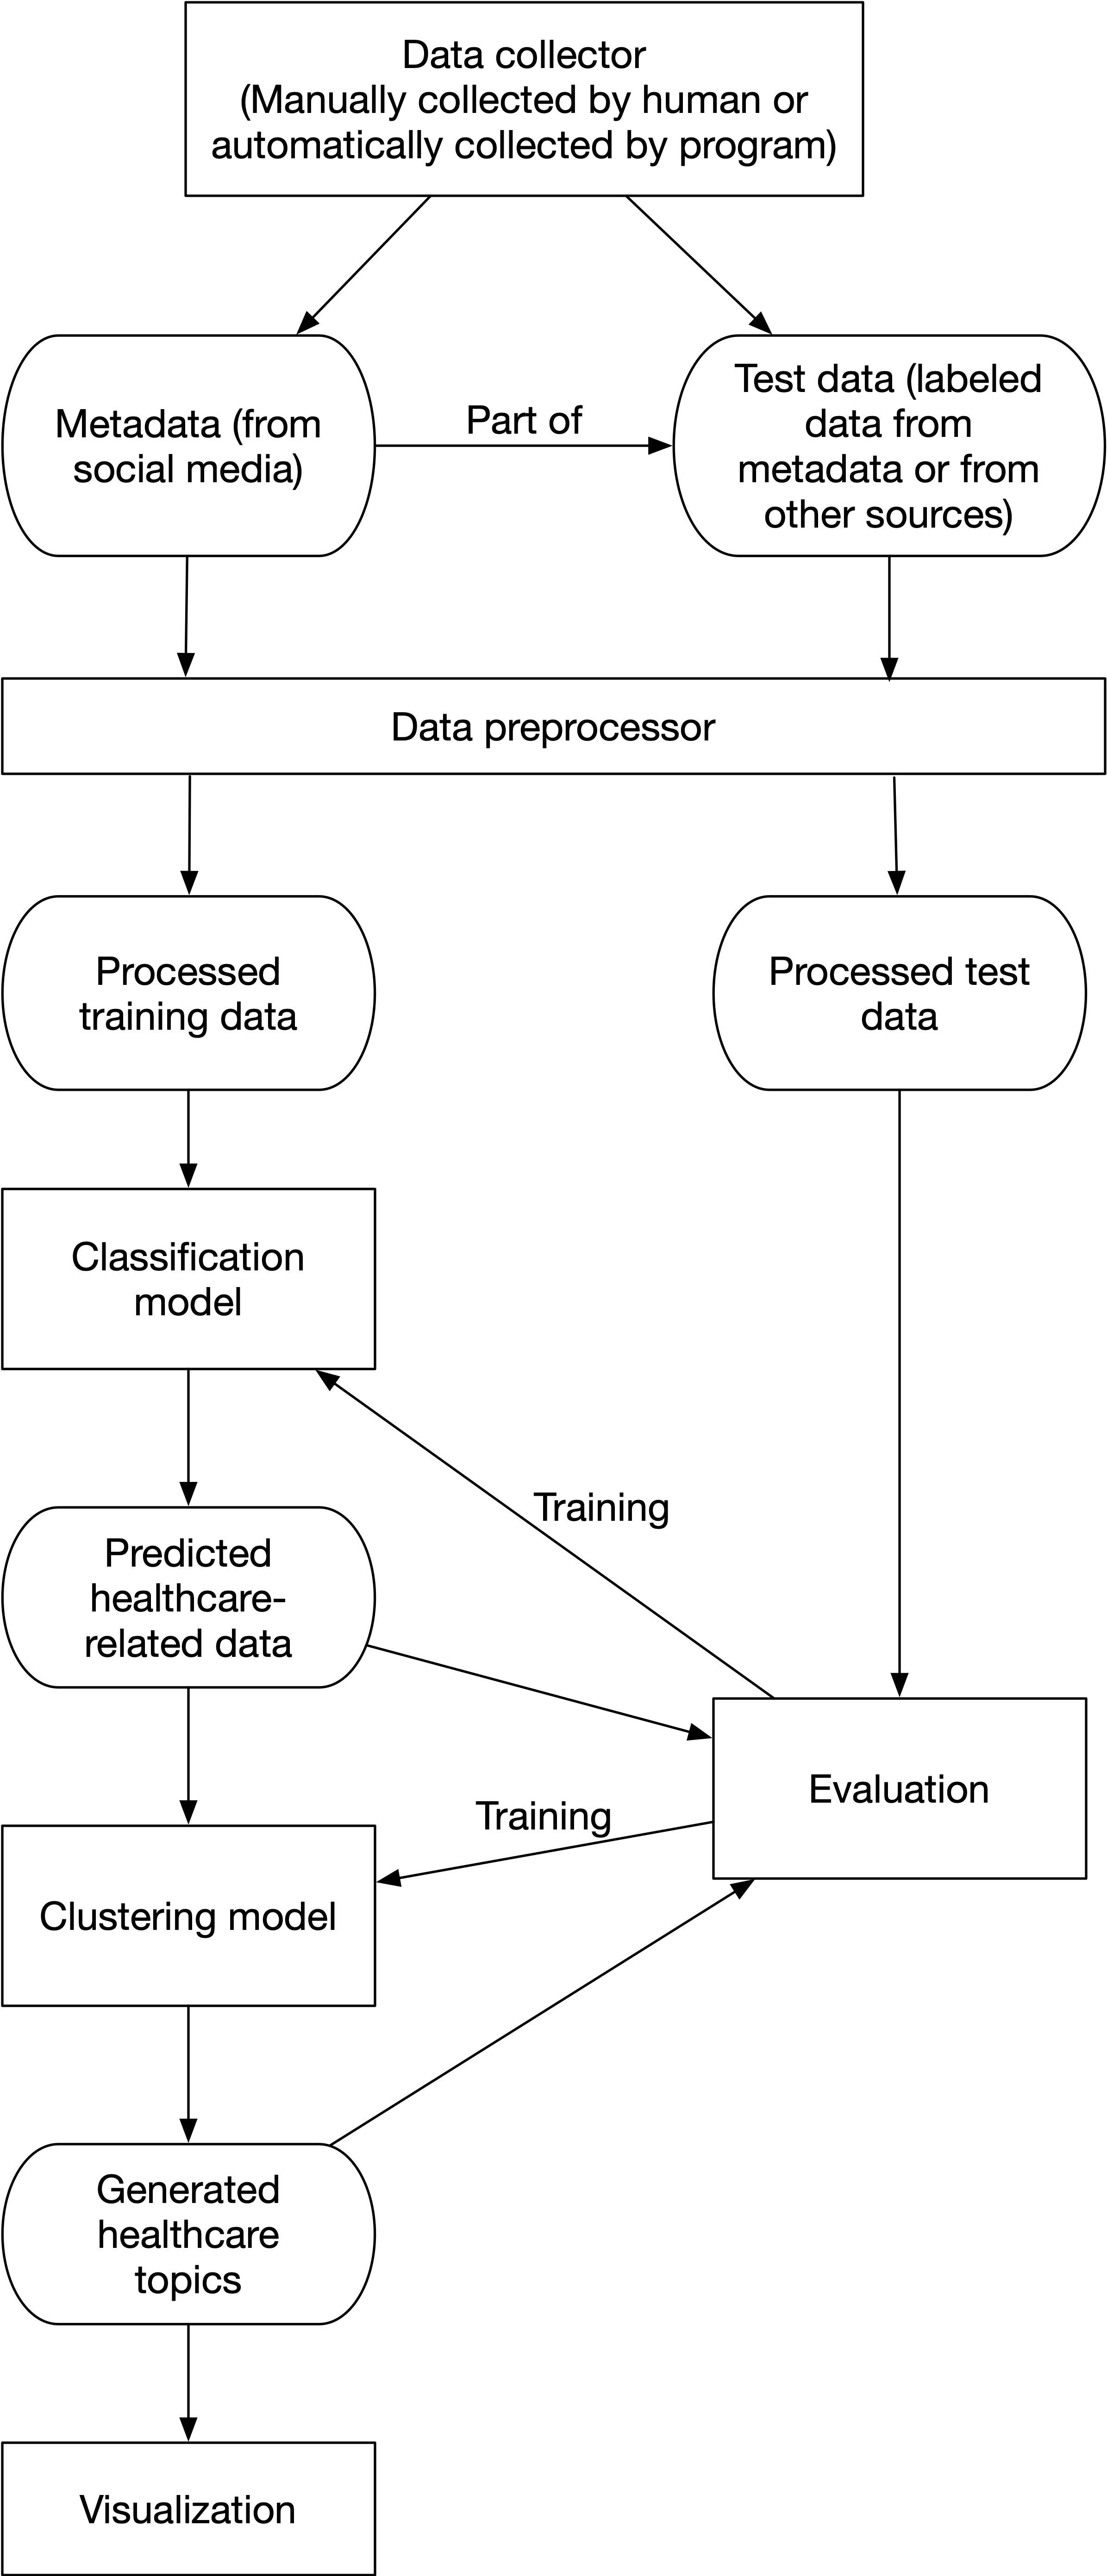
\includegraphics[width=3in]{sys2.jpg}
    \caption{Overall design}
    \label{fig:sys2}
\end{figure}
\section{Basic components}
This section show the preliminary design of our components, including the basic functional requirements of each part and the possible methods we may adopt. Following subsections represent stages(pipelines) of our system respectively, the general procedure design is inspired by \cite{feldman2007text}.
\subsection{Data collector design}
\label{sec:Data collector design}
Social media data is the input of the whole system, but according to the different social media platforms and various sources of data (such as extracted from official API or download from open-source dataset), the structure of data and methods of collecting data can be diverse. Therefore, we design an interface which can collect and integrate different metadata. In this project, we focus more on modeling and algorithm design rather than a complete system, therefore, we choose one certain social media platform. In addition, to evaluate the accuracy and performance of our model, we need a ground truth dataset (if available). Here the interface should at least collect these two dataset from at least one source respectively.\\
Functional requirements of this component are:
\begin{enumerate}
    \item Collect and store social media data from at least one source
    \item Collect and store ground truth data from at least one source, or manually label some data from metadata
\end{enumerate}
\subsection{Data preprocessor design}
\label{sec:Data preprocessor design}
Data collected by stage 1 are metadata, which could be unstructured and irrelevant to this project. We subdivide this step into smaller steps:
\begin{enumerate}
    \item Unify data structure: if one dataset comes from different sources (for example, facebook data extracted from API and from web spider). To pass these data into functions of later steps, a unified format is required. In addition, dataset could contain information that won't be used by our algorithm, ignore such information when unify data can save storage space. In our design, both unified structures of social media dataset and ground truth dataset should be implemented (see section \ref{sec:Data collection}). 
    \item Text regularization: social media dataset could adopt different coded format (such as ASCII and unicode), here we decide to use utf-8 encoding, which is wildly used in the Internet. The collected data could contain special symbols, unknown characters, URL links and emoji, pictures, videos (See Figure \ref{fig:tsc1}). In this project, we focus on pure text, thus information such as URL links, pictures and videos will be ignored. Inspired by \cite{serban2019real}, emoji and some pecial symbols can be transformed in to text based on standard transformation tables. We will adopt such transformation to keep maximum valuable data.
    \begin{figure}[!htp]
        \center
        
\includegraphics[width=4in]{images/tsc1.png}
        \caption{Tweet with URL and picture (screenshot from \href{https://twitter.com/search?q=flu&src=typed_query}{Twitter})}
        \label{fig:tsc1}
    \end{figure}
    \item Data filtering (classification): after the structuralization, the dataset can be used for analysis. However, not all the data contain information we want. This step will filter out irrelevant data of both social media dataset and ground truth dataset and reserve data that be considered useful. We will set inclusion rules and classifier to filter the data and label them (see section \ref{sec:Preprocessing}). The method we adopt to train a classifier is similar to how we build our prediction model. The detailed methods of text tokenization,encoding and building neural network model can be found in stage 3 of this section.
    \item Location extraction (possibly): in this project, we need data containing time of creation, geographic information to create our diffusion model. Data without such information can be used to train a classifier in the next step. The time of creation is contained in most sources (all the datasets we search so far provide temporal information). However, based on user's setting, some data don't contain geographic information (users can hide their private information if they wish). In addition, some platforms allow users name their own location (such as Wechat, users can assign personalized name to their location), or use a fake one. Platforms can adopt different standards of placename. Apart from that, even a user provide authentic private location, it still can't be guaranteed that he was in that place when posted tweets. All of such conditions bring noises in the dataset. Use the method we deal with unstructured metadata as reference, here we plan to the same solution: regularize the geographic information, set a standard in our project. In term of customized placename, we will design a function trying to map it to our standard (see Chapter 4). However, it worth noting that, the percent of social media with geographic information is comparably samll, which may not be sufficient to build a reliable predictive model (and this design could be changed based on it).
\end{enumerate}
Functional requirements of this component are:
\begin{enumerate}
    \item Must unify a data structure of social media dataset, and can integrate datasets (if more than one sources) into the same structure
    \item Must unify a data structure of ground truth datasets, and can integrate datasets (if more than one sources) into the same structure
    \item Must regularize all the text in the integrated dataset
    \item Must extract geographic information of each data if available
    \item Must regularize all the extracted geographic information into a unified format
\end{enumerate}
\subsection{Classification Model design}
\label{sec:First round predictor design}
As can be seen in figure \ref{fig:sys2}, the final model is designed as an ensemble of two models: a classification model and a clustering model. Classification model is help to screen out data that is irrelevant to healthcare, and hence we will use labeled data to fed it. Therefore, the model follows the the common process of solving NLP tasks.
\begin{enumerate}
    \item Text tokenization: neural network can only receive tensors as input, therefore, the first step of this stage is transforming the textual data into tensor, which is called tokenization (a token is a single unit extracted from text) \cite{Chollet:2017:DLP:3203489}. There are three basic word separation strategies: (1)split text into single words, transform each word into a vector; (2)split text into single character, transform each character into a vector; (3) extract n-gram of words or characters, transform each n-gram into a vector (a n-gram is a set of sequential words or characters), the resulting set is called bag-of-words \cite{Chollet:2017:DLP:3203489}. Bag-of-words can't record the order of words in the original text, therefore, this method is wildly used in shallow-layer model instead of deep learning model. Extracting n-gram is a feature engineering, which is inflexible and unstable. Here we adopt the first strategy, the feature extraction procedure will done by our deep learning model.
    \item Text encoding: the procedure that transform token into vector is called encoding. There are two most common methods. One is one-hot encoding, which assign each token a unique integer i, transform i into a binary vector (only contains 1 and 0) of length N (N is the size of token list), only the ith element is 1, others are 0. This method returns a high dimensional sparse vector (20000 dimensions or more), since each token takes one dimension. Anthoer encoding method is word embedding, which is learnt from dataset, returns a low dimensional intensive vector. The idea behind this method is that: the geometrical distance of two token should base on their relation (synonyms should have shorter distance than antonyms), and the vector's direction should have sense. For example, the vector of word ``king'' plus the vector of word ``female'' should return the vector of word ``queen'' \cite{Chollet:2017:DLP:3203489}. Therefore, we can't assign each token a vector randomly. In addition, for different tasks, the embedding space could be diverse, the embedding space used for sentiment analysis may not fit argot detection. In our design, we will try both of these two methods, and for the second, we will train a embedding space based on our dataset.
\end{enumerate}
\subsection{Clustering model design}
Some topics could be relatively new or have few samples, it's hard to label the classes of them in advance. Therefore, the classification model could not predict all minor topics related to healthcare. For this reason, we decide to use one more unsupervised model that helps to detect health events. Classification is in charge of deciding whether a given document contains information about healthcare, while the clustering model groups the filtered data in a time slice (such as in one day) and find the hidden topics. The functional requirements of this model are:
\begin{enumerate}
    \item Must take the filtered data from the classification model, and group them into clusters
    \item Must assign a interpretable topic to each cluster
    \item Must be evaluated by a criterion that correlates with human judgement
\end{enumerate}

\subsection{Evaluation layer design}
\label{sec:evaluation}
In our overall design (Figure \ref{fig:sys2}), there are two cycles linking this layer and two models respectively. This doesn't mean that those two model share the same evaluation criteria. In deed, this layer is abstract, it is designed to show that we will evaluate this two models respectively. 
\\\\For the supervised classification model, according to \cite{Chollet:2017:DLP:3203489}, there are 8 common methods can be adopted to evaluate the model: (1) confusion matrix; (2) accuracy; (3) precision; (4) recall; (5) F1 score; (6) ROC curve; (7) AUC (Area Under Curve); (8) PR curve. Especially, accuracy and recall are wildly used in class-imbalance problem (our task is class-imbalanced). Following are formulas of (2)(3)(4)(5), where TP, TN, FP, FN represents true positive (the number of cases correctly identified as required), ture negative the number of cases correctly identified as not required, false positive (the number of cases incorrectly identified as required), false negative (the number of cases incorrectly identified as not required), respectively:
\begin{displaymath}
    \begin{array}{c}
        Accuracy = \frac{TP+TN}{TP+FN+FP+TN} \\
        Precision = \frac{TP}{TP+FP}\\
        Recall = \frac{TP}{TP+FN}\\
        F1 = 2\times\frac{Precision \times Recall}{Precision + Recall}
    \end{array}
\end{displaymath}
Once the socre (target) is defined, we must adopt a method to assess the result. There are 3 common methods: (1) Hold-out method (test set estimation); (2) K-Fold Cross Validation; (3) Repeated k-fold Validation. The first method works by randomly divided dataset into two mutually exclusive subsets, the training set (often $\frac{2}{3} to \frac{4}{5}$ of the original set) and testing set. It is simple to implement but will be severely affected by the size of subsets. If the training instances is far more than testing instances, the evaluation result is unreliable, but in reverse, the model will lose fidelity. In addition, this method is unsuited to small sample sizes, since it can't make full use of data\cite{omary2010machine,Chollet:2017:DLP:3203489}. Second method partition data into k separate subsets of similar size. Each subset will be used as testing data in turns (k times) while left subsets will be used as training data, the final socre is the mean of all rounds. It can be regarded as a kind of hold-out method with the ability to exploit more data and provide higher reliability \cite{omary2010machine}. The third one is used when the available data are too fewer while high prediction accuracy is required. It repeat the second method and calculate average score \cite{Chollet:2017:DLP:3203489}.  \\
\\For the clustering model, there are several criteria, such as Silhouette Coefficient. However, we care more about the interpretability of generated topics rather than the grouped clusters. Here we decide to use coherence of topics to evaluate our model. The details can be found in section \ref{sec:unsupervised}.
Functional requirements of this component are:
\begin{enumerate}
    \item It should provide different evaluation indexes (Accuracy, Recall, etc.)to assess the prediction outcome.
    \item It should provide different evaluation methods (K-Fold, Hold-our, etc.) to assess the prediction outcome.
    \item Must choose a best combination of methods to evaluate prediction result based on ground truth dataset.
    \item Must set a baseline (or target) to stop training.
    \item The evaluation result must correlate with human judgement.
\end{enumerate}
\subsection{Visualization design}
The final result may not clear and meanful for users. Visualization can help users/researchers to figure out the potential information of data/result, such as its feature, pattern, trend and relationship \cite{grinstein2002information}. There are various visualization techniques for different sceniros, purposes and data/input, such as 2D display (bar chart) and 3D display (cloud vapor), in addition, if the prediction is real-time, the visualization could be dynamic.  In this project, visualization is used in the last stage, therefore, we can assume the the input is stable and predictable. In addition, the prediction is numerical, according to \cite{grinstein2002information}, geometric representing methods could be used, such as scatetr plot, lines etc. The final method will be adopted based on the experimental result.\\\\
Functional requirements of this component includes:
\begin{enumerate}
    \item It should integrate the whole process and choose an approach to display the result.
    \item It should ignore uninterpretable or ambiguous topics. 
\end{enumerate}